\subsection{Riesgos del modelo clásico}

La seguridad de NFS debe analizarse en capas. El protocolo puede ejecutarse sobre una red privada, pero eso no implica que sea automaticamente seguro. El modelo tradicional \texttt{AUTH\_SYS} confia en los UID y GID que informa el cliente. Si un atacante obtiene privilegios de administrador en un cliente autorizado, puede intentar presentar identidades numericas que no le corresponden.

Otro riesgo es la autorizacion basada unicamente en IP o subred. Restringir exports por direccion es necesario, pero no suficiente. En una red comprometida, un atacante podria intentar suplantar una IP autorizada o aprovechar una configuracion demasiado amplia, por ejemplo exports disponibles para \texttt{*}. A esto se suma que, sin cifrado, los datos y metadatos pueden viajar en claro.

\subsection{Control por IP, subred y firewall}

La primera capa de defensa consiste en publicar cada export solo a los clientes que realmente lo necesitan. En \texttt{/etc/exports} pueden indicarse hosts concretos, subredes o grupos administrados. A nivel de red, los firewalls deben permitir unicamente el trafico necesario. Para NFSv4, esto significa principalmente TCP 2049 entre clientes autorizados y servidor. Si se habilita NFSv3, deben contemplarse tambien sus servicios auxiliares.

La segmentacion mediante VLAN de almacenamiento reduce exposicion lateral. Sin embargo, no reemplaza autenticacion ni permisos. Una VLAN dedicada controla quien puede llegar al servicio; los permisos y mecanismos criptograficos controlan que puede hacer cada identidad una vez que llega.

\subsection{\texttt{root\_squash} e identidades}

Una proteccion fundamental es \texttt{root\_squash}. Con esta opcion, las solicitudes provenientes del usuario root de un cliente no se ejecutan como root en el servidor, sino que se mapean a un usuario anonimo, comunmente \texttt{nobody}. Esto evita que el administrador local de un cliente tenga automaticamente control total sobre los archivos exportados por el servidor.

El control de acceso tambien depende de la coherencia de identidades. Si el UID 1000 representa usuarios distintos en dos equipos, los permisos pueden volverse inconsistentes. En NFSv4, servicios como \texttt{idmapd} pueden mapear identidades de red hacia usuarios locales, idealmente respaldadas por LDAP, FreeIPA o Active Directory.

\subsection{Kerberos, TLS y buenas prácticas}

NFSv4 incorpora soporte para autenticacion fuerte mediante RPCSEC\_GSS, habitualmente con Kerberos. Los modos \texttt{sec=krb5}, \texttt{sec=krb5i} y \texttt{sec=krb5p} agregan autenticacion, integridad y privacidad respectivamente. El modo mas seguro introduce mayor sobrecarga, por lo que debe elegirse segun el tipo de dato y el modelo de amenaza.

Tambien existe RPC sobre TLS, formalizado en RFC 9289, como mecanismo moderno para aportar cifrado de transporte. Su adopcion depende del soporte de cada sistema operativo y distribucion, por lo que debe considerarse una opcion a evaluar, no un reemplazo universal inmediato.

\begin{figure}[H]
    \centering
    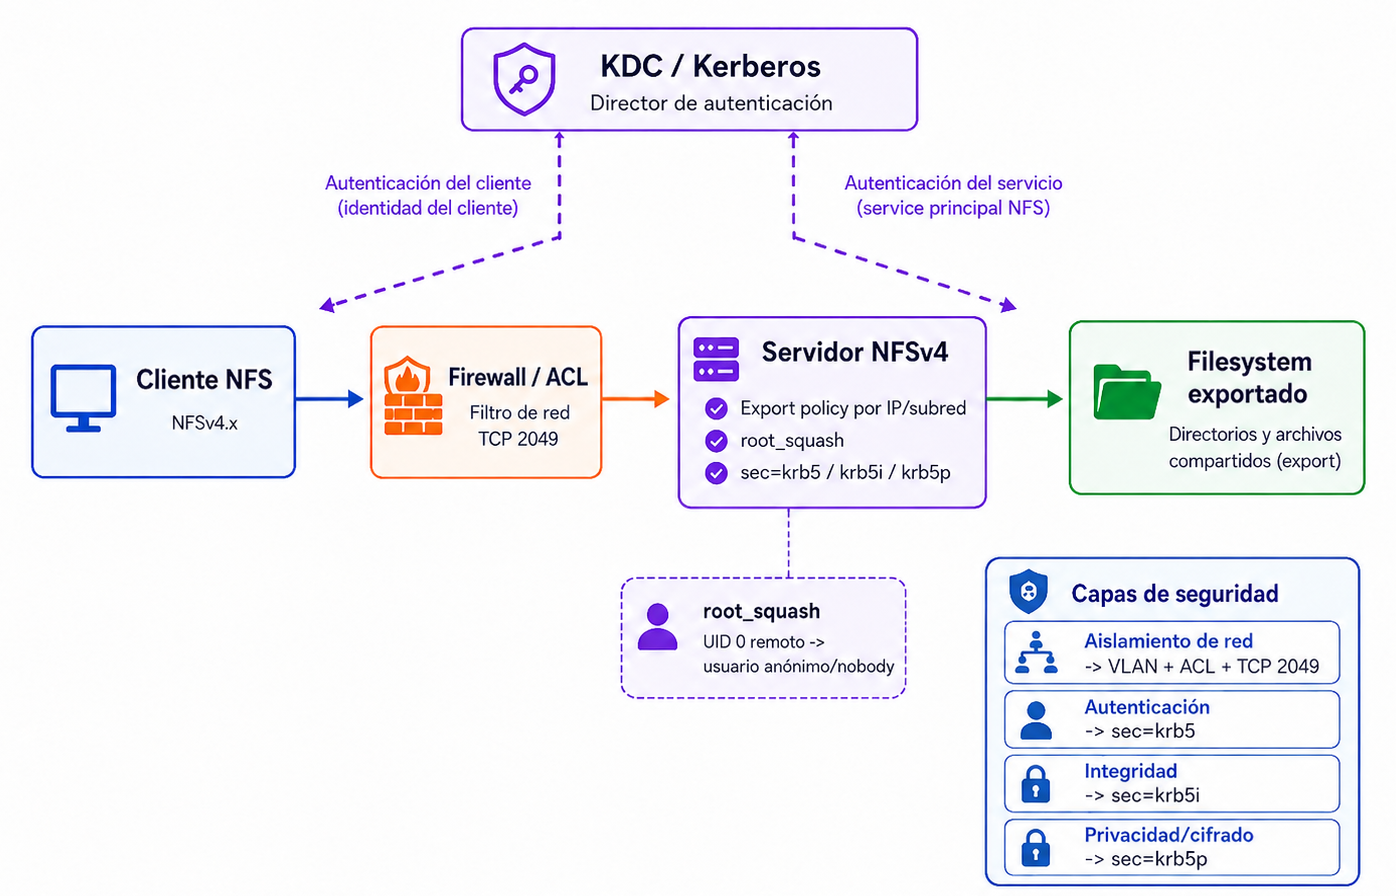
\includegraphics[width=0.95\textwidth]{img/nfs_04.png}
    \caption{Seguridad en NFS}
    \label{fig:nfs_seguridad_capas}
\end{figure}

Como buenas practicas generales, un despliegue NFS en datacenter deberia usar NFSv4.1 o superior, filtrar TCP 2049 por subred, evitar exports globales, mantener \texttt{root\_squash}, separar el trafico en una VLAN dedicada y aplicar Kerberos o TLS cuando el tipo de dato lo justifique.
